\subsection{Alternative to Estimate $\hat{\textbf{A}}$}  
As concluded does the implementation of Cov-DL not provide a sufficient estimate of the mixing matrix $\mathbf{A}$. 
Therefore a different approach is necessary. 

Replacing the insufficient estimate by a fixed estimate $\hat{\mathbf{A}}_{\text{fix}}$ is one immediately solution. By the term fixed one referrers to the estimate being manual chosen rather than being data dependent.  
This choice is supported by the observations from Cov-DL2 where $\mathbf{A}_{\text{init}}$ matrix provides an estimate which happens to be at least as good as the one provided by Cov-DL. 
Thus, the challenge is now to choose a fixed matrix for which its characteristics resemble those of the true mixing matrix. 
However, from chapter \ref{ch:motivation} it is clear that no specific characteristics of the mixing matrix are known, which supports the choice of a random matrix of Gaussian distribution or similar, as it was chosen for the initial guess $\mathbf{A}_{\text{init}}$.
By randomly generating the fixed estimated, an estimate is drawn from the specific distribution. Thus different realizations occur for every data set.    
From this perspective three fixed estimates of the mixing matrix are defined, by drawing each entry from a specified distribution: 
\begin{itemize}
\item[] $\hat{\mathbf{A}}_{\text{uni}} \sim \mathcal{U}(-1,1)$
\item[] $\hat{\mathbf{A}}_{\text{norm1}} \sim \mathcal{N}(0,1)$                                           
\item[] $\hat{\mathbf{A}}_{\text{norm2}} \sim \mathcal{N}(0,2)$ 
\end{itemize}
Note that the second matrix $\hat{\mathbf{A}}_{\text{norm1}}$ is generated the same way as the true mixing matrix of the stochastic data set, being a different realization. 
Thus, $\hat{\mathbf{A}}_{\text{norm1}}$ is expected to have the lowest MSE when compared to the true mixing matrix $\mathbf{A}$. 
However, it is of interest to investigate whether it is the best estimate of $\mathbf{A}$ which provide the best estimate of $\mathbf{X}$. 

A different option regarding a choice for a fixed estimate $\hat{\mathbf{A}}_{\text{fix}}$ is to utilize the ICA algorithm, described in appendix \ref{app:ICA}. 
By the ICA algorithm it is possible to solve the EEG inverse problem for both $\mathbf{A}$ and $\mathbf{X}$, in the case where $k \leq M$.
Consider a simulation of a stochastic data set specified by $N = k = M$. 
Solving the system by ICA yields an estimate of $\mathbf{A}$. 
Now reduce the data set $\mathbf{Y}$ such that $M \leq k$. 
Similar the estimate of $\mathbf{A}$ is reduced by removing the same rows as in $\mathbf{Y}$. 
This yields an estimate $\hat{\mathbf{A}}_{\text{ICA}}$ which can be used as a fixed input to M-SBL along with the corresponding reduced $\mathbf{Y}$.

The four different fixed estimates $\hat{\mathbf{A}}_{\text{fix}}$ are tested on the stochastic data set specified by $M = 10$, $N = k = 16$ and $L = 1000$. 
As a reference the true mixing matrix $\mathbf{A}$ is included in the plot, to see the best possible $\text{MSE}(\mathbf{X}, \hat{\mathbf{X}})$.
To get an average performance 50 different simulations are conducted with the same specifications. For each system $\mathbf{X}$ is estimated from each of the four fixed estimates\footnote{Note that for each of the 50 repetitions four different realizations of $\hat{\mathbf{A}}_{\text{fix}}$ are fixed.} of $\mathbf{A}$, and the corresponding MSE is computed. 
The resulting average $\text{MSE}(\mathbf{A}, \hat{\mathbf{A}}_{\text{fix}})$ and $\text{MSE}(\mathbf{X}, \hat{\mathbf{X}})$ are visualized in figure \ref{fig:vary_A}, for each of the four $\hat{\mathbf{A}}_{\text{fix}}$. 
Furthermore, the plotted values are found in table \ref{tab:fixed}.
\begin{figure}[H]
\centering
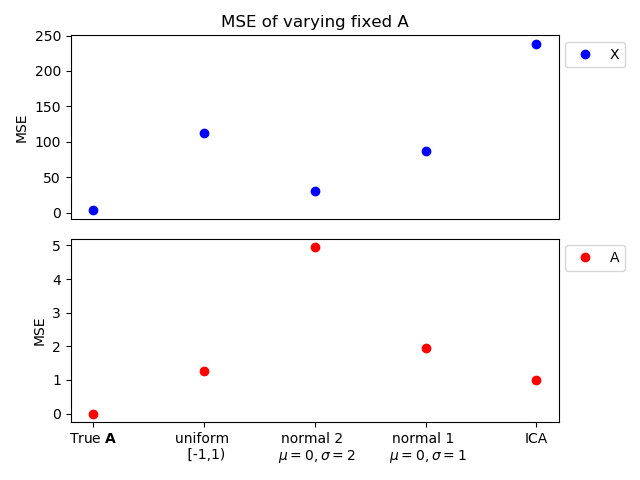
\includegraphics[scale=0.5]{figures/ch_6/A_fix1.png}
\caption{Average MSE($\textbf{A},\hat{\mathbf{A}}$) value for each of the four fixed estimates $\hat{\mathbf{A}}_{\text{fix}}$ and the corresponding MSE$(\textbf{X},\hat{\mathbf{X}})$. From a stochastic data set specified by $M = 10$, $N = k = 16$ and $L = 1000$.}
\label{fig:vary_A}
\end{figure}
\noindent
%
%\begin{table}[H]
%\centering
%\begin{tabular}{|c|c|c|c|c|c|}
%\hline
% &  $\mathbf{A}$ & $\hat{\mathbf{A}}_{\text{uni}}$ & $\hat{\mathbf{A}}_{\text{norm2}}$	 & $\hat{\mathbf{A}}_{\text{norm1}}$ & $\hat{\mathbf{A}}_{\text{ICA}}$ \\
%\hline
%$\text{MSE}(\mathbf{A}, \hat{\mathbf{A}})$ & 0 & 1.271 & 4.957 & 1.941 & 1.006 \\
%\hline
%$\text{MSE}(\mathbf{X}, \hat{\mathbf{X}})$ & 3.271 & 113.10 & 30.02 & 86.51 & 238.5 \\
%\hline
%\end{tabular}
%\caption{Average MSE values resulting from stochastic data set specified by $M = 10$, $N = k = 16$ and $L = 1000$ with a fixed estimate of the mixing matrix $\hat{\mathbf{A}}_{\text{fix}}$.}
%\label{tab:fixed}
%\end{table}
%\noindent
From figure \ref{fig:vary_A} it is first of all seen that relation between the MSE of $\mathbf{A}$ and $\mathbf{X}$ do not behave as expected. The lowest $\text{MSE}(\mathbf{A}, \hat{\mathbf{A}}_{\text{fix}})$ results in the highest $\text{MSE}(\mathbf{X}, \hat{\mathbf{X}})$ and so forth. 
The lowest $\text{MSE}(\mathbf{A}, \hat{\mathbf{A}}_{\text{fix}})$ is achieved by using $\hat{\mathbf{A}}_{\text{ICA}}$, which confirms that the ICA algorithm manages to estimate $\mathbf{A}$ when $k \leq M$. 
However, as this do not result in the best estimate of $\mathbf{X}$ a different choice of $\hat{\mathbf{A}}_{\text{fix}}$ is still considered. 
The lowest $\text{MSE}(\mathbf{X}, \hat{\mathbf{X}})$ is achieved by use of $\hat{\mathbf{A}}_{\text{norm2}}$, which resulted in the largest $\text{MSE}(\mathbf{A}, \hat{\mathbf{A}}_{\text{fix}})$. 
      
As the main interest in this thesis is to identify the active sources of EEG measurements, a low $\text{MSE}(\mathbf{X}, \hat{\mathbf{X}})$ is more desirable than a low $\text{MSE}(\mathbf{A}, \hat{\mathbf{A}}_{\text{fix}})$. 
Furthermore, a disadvantage of using $\hat{\mathbf{A}}_{\text{ICA}}$ is the limitations in practice when $k = M$ is not possible. 
From these observations a fixed estimate of the mixing matrix drawn from a normal distribution with mean 0 and variance 2, is chosen as the alternative estimate of $\mathbf{A}$. 
Thus is it concluded that $\hat{\mathbf{A}}_{\text{fix}} := \hat{\mathbf{A}}_{\text{norm2}}$ will replace the Cov-DL stage in the main algorithm, cf. figure \ref{fig:flow}, throughout the remaining parts of this thesis. 

Due to the unexpected relation between MSE$(\mathbf{A}, \hat{\mathbf{A}}_{\text{fix}})$ and $\text{MSE}(\mathbf{X}, \hat{\mathbf{X}})$ an additional investigation is conducted. 
Figure \ref{fig:X_func_SNR} shows the $\text{MSE}(\mathbf{X}, \hat{\mathbf{X}})$ as a function of the mixing matrix $\mathbf{A}$ with varying SNR. 
Specifically white noise $\textbf{W}(\text{SNR})$ is added to the true mixing matrix depending on the desired SNR, such that 
\begin{align*}
\hat{\textbf{A}} = \textbf{A}+\textbf{W}(\text{SNR}).
\end{align*}
The SNR is considered in the interval $[0.01, 2]$. 
For each SNR 100 simulations are performed an the average $\text{MSE}(\mathbf{X}, \hat{\mathbf{X}})$ is computed.
Additionally figure \ref{fig:A_func_SNR} shows the corresponding average $\text{MSE}(\mathbf{A}, \hat{\mathbf{A}})$.

From figure \ref{fig:X_func_SNR} it is seen that MSE decreases as the SNR increases. 
This indicates as first expected that the better estimate of the true mixing matrix $\mathbf{A}$ the better estimate of source matrix $\mathbf{X}$. 
However, this is still a contradiction to the result seen in figure \ref{fig:vary_A}. 
This could possible correspond to true mixing matrix $\mathbf{A}$ being a Gaussian matrix with $\mu = 0$ and $\sigma = 1$ for which Gaussian noise is added. 
The average $\text{MSE}(\mathbf{A}, \hat{\mathbf{A}})$ seen in figure \ref{fig:A_func_SNR} is seen to be far below 1 even for a large amount of noise, which is remarkably lower than the MSE values previously seen in figure \ref{fig:vary_A}\todo{begge plot titles skal ændres, hat på A}.  
\begin{figure}[H]
\begin{widepage}
    \begin{minipage}[t]{.45\textwidth}
    	\centering
		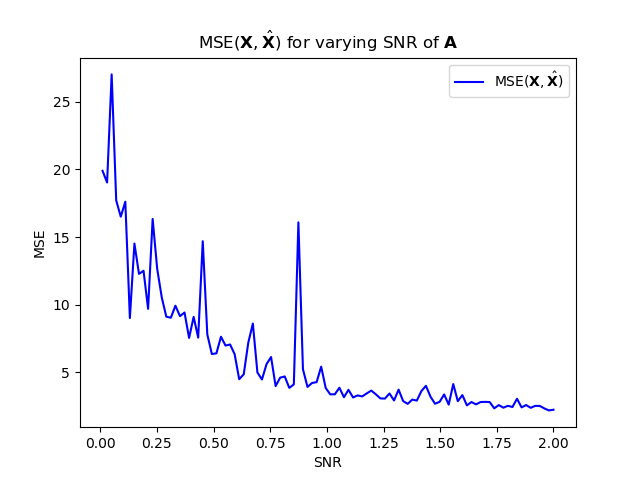
\includegraphics[scale=0.5]{figures/ch_6/X_func_SNR.png}
		\caption{MSE$(\mathbf{X},\hat{\mathbf{X}})$ estimated from stochastic data set specified by $M = 6$, $N = k = 8$ and $L = 1000$, as a function of SNR of given $\hat{\mathbf{A}}$.}
		\label{fig:X_func_SNR}
    \end{minipage} 
    \hspace{0.5cm}
    \begin{minipage}[t]{.45\textwidth}
        \centering
		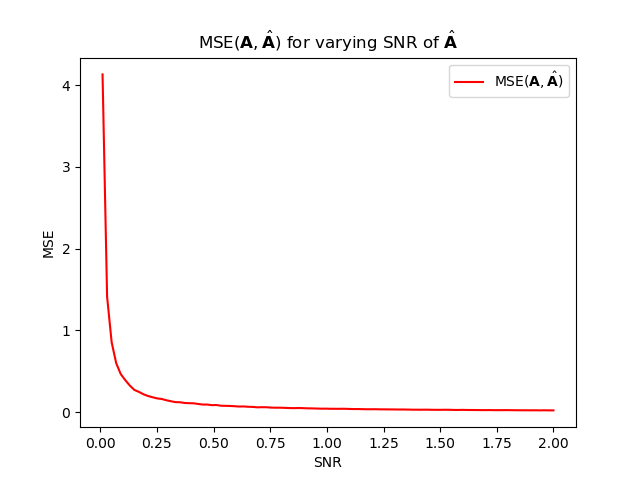
\includegraphics[scale=0.5]{figures/ch_6/A_func_SNR.png}
		\caption{MSE$(\mathbf{A}, \hat{\mathbf{A}})$ where $\hat{\mathbf{A}}$ is a function of the SNR. $\hat{\mathbf{A}}$ correspond to $\hat{\mathbf{A}}$ used in figure \ref{fig:X_func_SNR}.}
		\label{fig:A_func_SNR}
    \end{minipage}
\end{widepage}
\end{figure}
\noindent